\section{Introduction to Planning and Control}

The previous chapters were about \emph{perception}: understanding where the vehicle is and what is around it. From this chapter on we move to the second half of the autonomous driving stack: deciding \emph{what to do} (\textbf{planning}) and \emph{how to do it} with the actuators (\textbf{control}).

\subsection{Basic terminology}
Some terms are used with a precise meaning in planning and control:
\begin{compactitemize}
    \item \textbf{Position}: the specific location of a point in space, usually given by its coordinates (e.g.\ $x, y, z$) in a 2D or 3D space.
    \item \textbf{Pose}: the position \emph{and} the orientation of a robot or of one of its parts.
    \item \textbf{Path}: a set of points in space that should be tracked. It says \emph{where} to go, but not \emph{when}.
    \item \textbf{Speed profile}: a set of velocities to be tracked, one for each point of the path.
    \item \textbf{Trajectory}: a path together with a speed profile. It can also be defined as a \textbf{path over time}, since knowing the speed at every point tells us when each point is reached.
\end{compactitemize}

\subsection{The autonomous driving paradigm}
An autonomous driving system is usually organized in three stages, \textbf{Perceive}, \textbf{Plan} and \textbf{Act}, which run on top of the hardware (sensors, computing platform and actuators):
\begin{compactitemize}
    \item \textbf{Perceive}: sensor processing, sensor fusion, object detection and tracking, localization and mapping. This is what we studied in the first part of the course;
    \item \textbf{Plan}: global planning, behavioural decisions and local planning;
    \item \textbf{Act}: control, which sends the commands to the vehicle.
\end{compactitemize}

\begin{figure}[H]
    \centering
    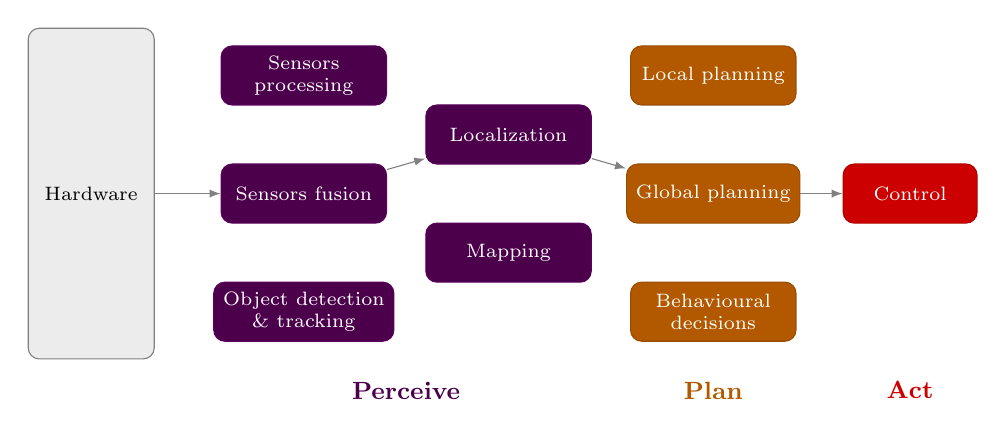
\begin{tikzpicture}[
        font=\scriptsize, >=latex,
        perc/.style={draw=violet!70!black, fill=violet!60!black, text=white, rounded corners, minimum width=2.1cm, minimum height=0.75cm, align=center},
        plan/.style={draw=orange!60!black, fill=orange!70!black, text=white, rounded corners, minimum width=2.1cm, minimum height=0.75cm, align=center},
        act/.style={draw=red!70!black, fill=red!80!black, text=white, rounded corners, minimum width=1.7cm, minimum height=0.75cm, align=center}]
        \node[draw=gray, fill=gray!15, rounded corners, minimum width=1.6cm, minimum height=4.2cm] (hw) at (0,0) {Hardware};
        \node[perc] (sp) at (2.7,1.5) {Sensors\\processing};
        \node[perc] (sf) at (2.7,0) {Sensors fusion};
        \node[perc] (od) at (2.7,-1.5) {Object detection\\\& tracking};
        \node[perc] (lo) at (5.3,0.75) {Localization};
        \node[perc] (ma) at (5.3,-0.75) {Mapping};
        \node[plan] (lp) at (7.9,1.5) {Local planning};
        \node[plan] (gp) at (7.9,0) {Global planning};
        \node[plan] (bd) at (7.9,-1.5) {Behavioural\\decisions};
        \node[act] (co) at (10.4,0) {Control};
        \draw[->, gray] (hw) -- (sf);
        \draw[->, gray] (sf) -- (lo);
        \draw[->, gray] (lo) -- (gp);
        \draw[->, gray] (gp) -- (co);
        \node[violet!60!black, font=\small\bfseries] at (4,-2.5) {Perceive};
        \node[orange!70!black, font=\small\bfseries] at (7.9,-2.5) {Plan};
        \node[red!80!black, font=\small\bfseries] at (10.4,-2.5) {Act};
    \end{tikzpicture}
    \caption{The Perceive--Plan--Act paradigm of autonomous driving}
\end{figure}

\subsection{Plan and Act}
Let's zoom in on the Plan and Act stages. They are split into a chain of modules, from the most abstract (where to go) to the most concrete (how much current to send to a motor), as shown in Figure~\ref{fig:plan-act}.

\begin{figure}[H]
    \centering
    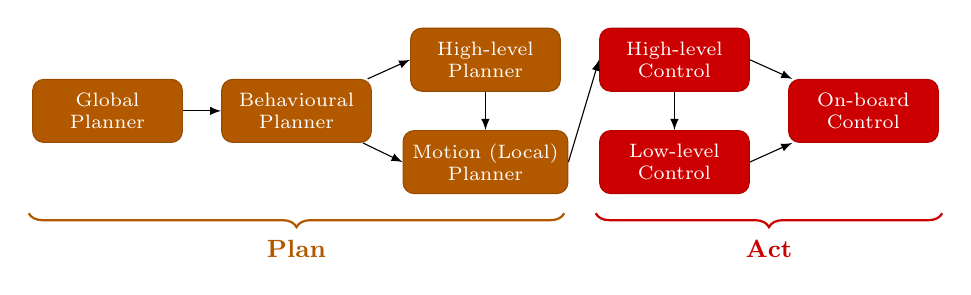
\begin{tikzpicture}[
        font=\scriptsize, >=latex,
        plan/.style={draw=orange!60!black, fill=orange!70!black, text=white, rounded corners, minimum width=1.9cm, minimum height=0.8cm, align=center},
        act/.style={draw=red!70!black, fill=red!80!black, text=white, rounded corners, minimum width=1.9cm, minimum height=0.8cm, align=center}]
        \node[plan] (gp) at (0,0) {Global\\Planner};
        \node[plan] (bp) at (2.4,0) {Behavioural\\Planner};
        \node[plan] (hp) at (4.8,0.65) {High-level\\Planner};
        \node[plan] (mp) at (4.8,-0.65) {Motion (Local)\\Planner};
        \node[act] (hc) at (7.2,0.65) {High-level\\Control};
        \node[act] (lc) at (7.2,-0.65) {Low-level\\Control};
        \node[act] (oc) at (9.6,0) {On-board\\Control};
        \draw[->] (gp) -- (bp);
        \draw[->] (bp) -- (hp.west);
        \draw[->] (bp) -- (mp.west);
        \draw[->] (hp) -- (mp);
        \draw[->] (mp.east) -- (hc.west);
        \draw[->] (hc) -- (lc);
        \draw[->] (hc.east) -- (oc);
        \draw[->] (lc.east) -- (oc);
        \draw[orange!70!black, thick, decorate, decoration={brace, mirror, amplitude=5pt}] (-1,-1.3) -- (5.8,-1.3) node[midway, below=6pt, font=\small\bfseries] {Plan};
        \draw[red!80!black, thick, decorate, decoration={brace, mirror, amplitude=5pt}] (6.2,-1.3) -- (10.6,-1.3) node[midway, below=6pt, font=\small\bfseries] {Act};
    \end{tikzpicture}
    \caption{The modules of planning (orange) and control (red)}\label{fig:plan-act}
\end{figure}

\subsubsection{Planning}
\textbf{Planning} is the task of deciding the high-level actions to take and of creating a \textbf{reference} to be followed. It is made of four modules:
\begin{compactitemize}
    \item \textbf{Global planner}: it generates a trajectory from a point A to a point B \emph{without} considering dynamic moving objects. It is like the route computed by a navigator.
    \item \textbf{Behavioural planner}: it decides which high-level actions to take, such as responding to traffic lights, respecting traffic rules and applying high-level safety logics (e.g.\ stop, overtake, give way).
    \item \textbf{High-level planner}: it defines the available \textbf{free space}, or limits the final plan, according to what the behavioural planner decided. For example, if the decision is ``do not overtake'', it removes the space of the other lane.
    \item \textbf{Local motion planner}: it generates the \textbf{final trajectory}, starting from the one produced by the global planner and taking into account the other modules and the static or moving obstacles nearby.
\end{compactitemize}

\subsubsection{Control}
\textbf{Control} generates the commands needed to \textbf{track the reference} (a trajectory) produced by the planner. It is made of three modules:
\begin{compactitemize}
    \item \textbf{High-level control}: it generates the commands to move the vehicle, such as \textbf{throttle, brake and steer}.
    \item \textbf{Low-level control}: it applies the control related to the vehicle dynamics, such as Traction Control (TC), Anti-lock Braking System (ABS), Electronic Stability Control (ESC) and Torque Vectoring.
    \item \textbf{On-board control}: it controls the on-board \textbf{actuators} to execute the requested steer, throttle and brake commands.
\end{compactitemize}

In practice these three blocks are often \textbf{combined}, or some of them are neglected. For example, high-level and low-level control can be merged into a single controller that directly produces the final throttle, brake and steer commands.

\subsection{Planning and control approaches}
There are several approaches and philosophies to design planning and control, for example:
\begin{compactitemize}
    \item \textbf{separating or combining} the \textbf{longitudinal} problem (speed, i.e.\ throttle and brake) and the \textbf{lateral} problem (steering) in the planning and/or control modules;
    \item \textbf{vehicle model-based} planning and control, which use a mathematical model of the vehicle dynamics;
    \item controlling the system as a \textbf{black box}, without an explicit model;
    \item \textbf{graph-based} motion planning.
\end{compactitemize}
For simplicity, in this course the \textbf{longitudinal and lateral problems are kept separate}, and we will see both vehicle model-based algorithms and more heuristic ones.

\subsection{Frameworks and tools}
\textbf{Matlab/Simulink.} It follows the \textbf{Model-Based Design} (MBD) development paradigm: the system is designed and simulated as a model, and the code is generated from it. The \emph{Automated Driving Toolbox} offers ready-made blocks for sensors, scenarios and planning.

\textbf{Autoware/ROS2.} \textbf{Autoware} is an \textbf{open-source} software stack for autonomous driving, maintained by the Autoware Foundation and built on top of \textbf{ROS2}.

\begin{figure}[H]
    \centering
    \begin{subfigure}[b]{0.46\textwidth}
        \centering
        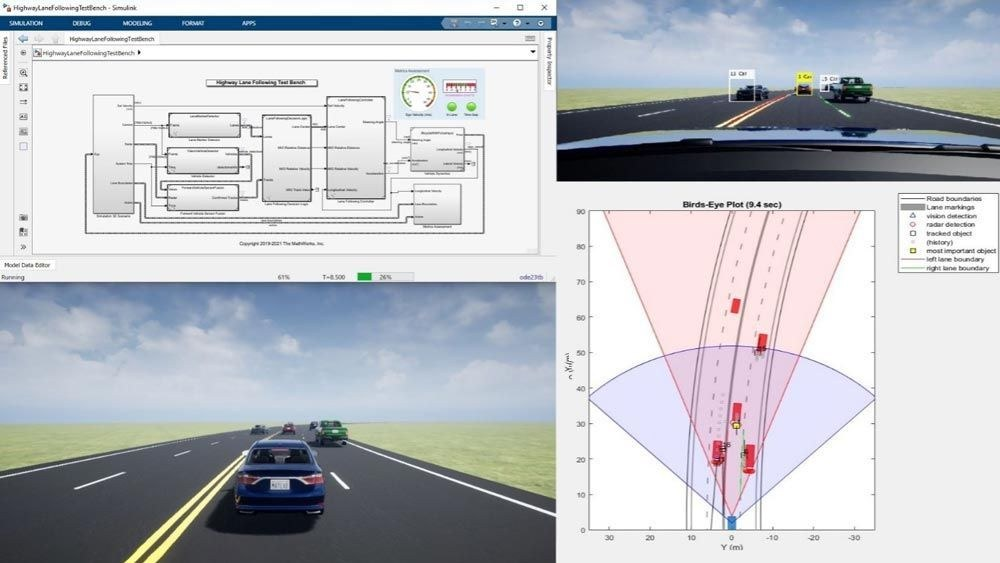
\includegraphics[height=4cm]{images/C13_1.jpg}
        \caption{Matlab Automated Driving Toolbox}
    \end{subfigure}
    \hfill
    \begin{subfigure}[b]{0.46\textwidth}
        \centering
        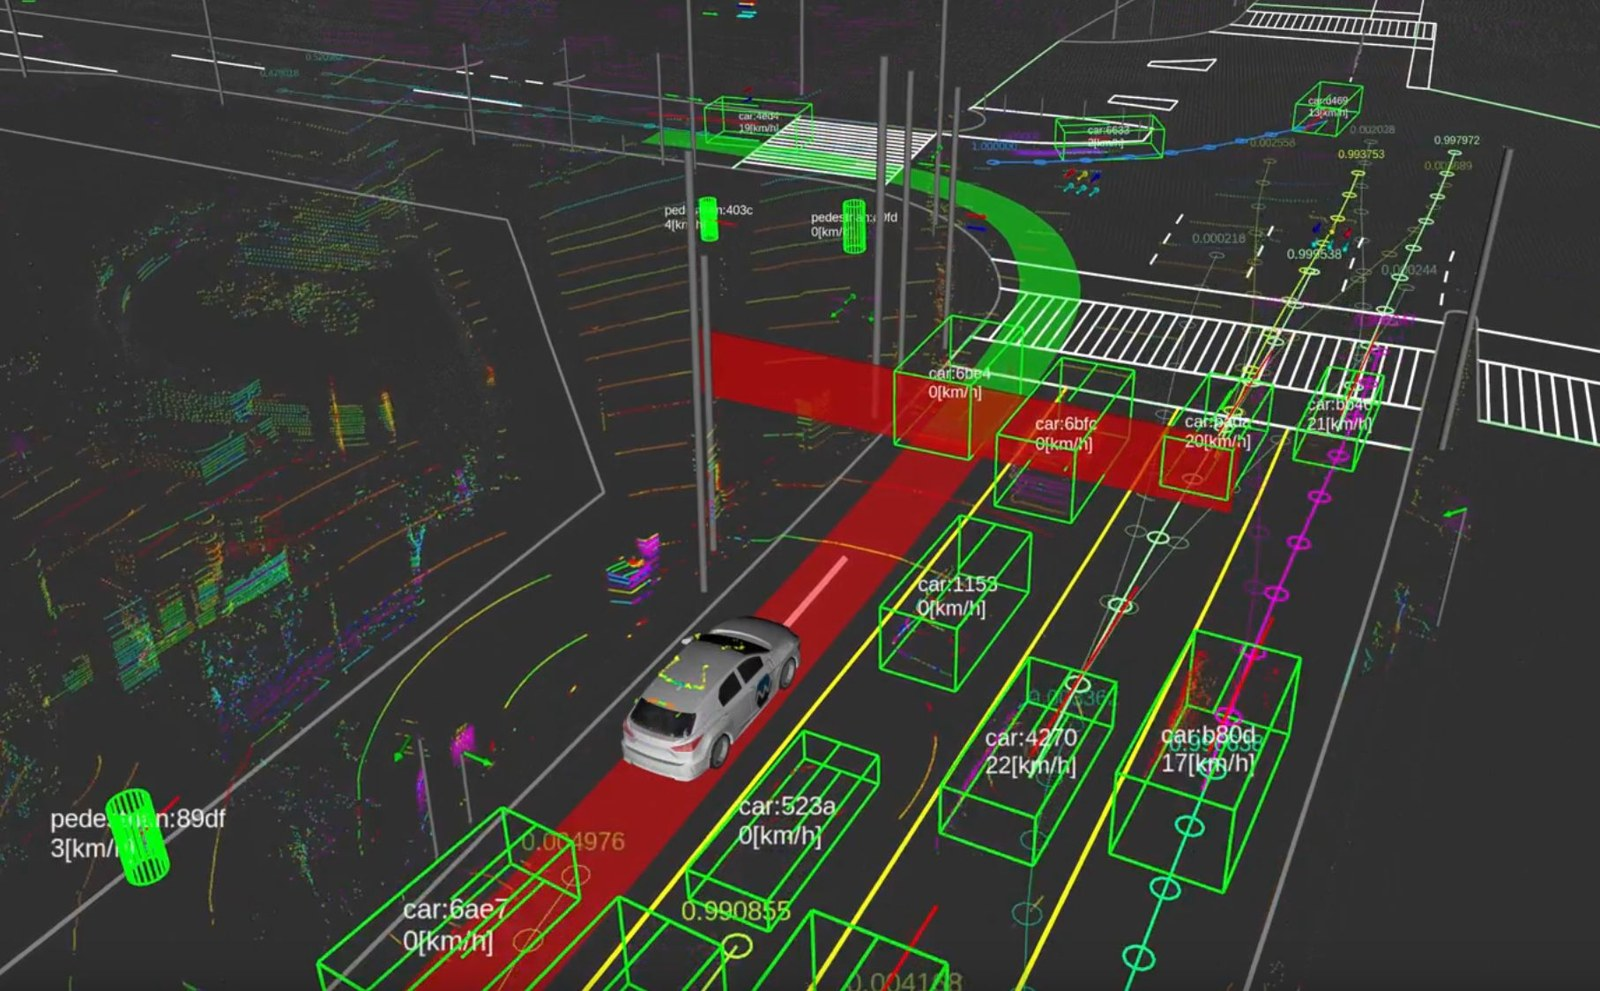
\includegraphics[height=4cm]{images/C13_2.jpg}
        \caption{Autoware}
    \end{subfigure}
    \caption{Two frameworks for planning and control}
\end{figure}

\textbf{Custom C++ software.} Planning and control modules can also be custom-made in C++:
\begin{compactitemize}
    \item \textbf{pros}: they can (potentially) satisfy the requirements of \textbf{real-time systems}, and the design and implementation are tailored to the final application;
    \item \textbf{cons}: they are not for beginners, and they are more prone to bugs and errors, at least in the short term.
\end{compactitemize}
Examples of open-source custom software stacks are \textbf{comma.ai openpilot} and \textbf{Apollo} (Baidu).

\subsection{Real autonomous driving applications}
\textbf{Urban cars: robotaxis.} Several robotaxi services are active in the USA and in China, e.g.\ \textbf{Waymo}, \textbf{Zoox}, \textbf{Cruise} and \textbf{Tesla Robotaxi}.

\textbf{Last-minute delivery.} Autonomous vehicles such as drones, robots or self-driving vans provide rapid, on-demand delivery for urgent needs.

\begin{figure}[H]
    \centering
    \begin{subfigure}[b]{0.24\textwidth}
        \centering
        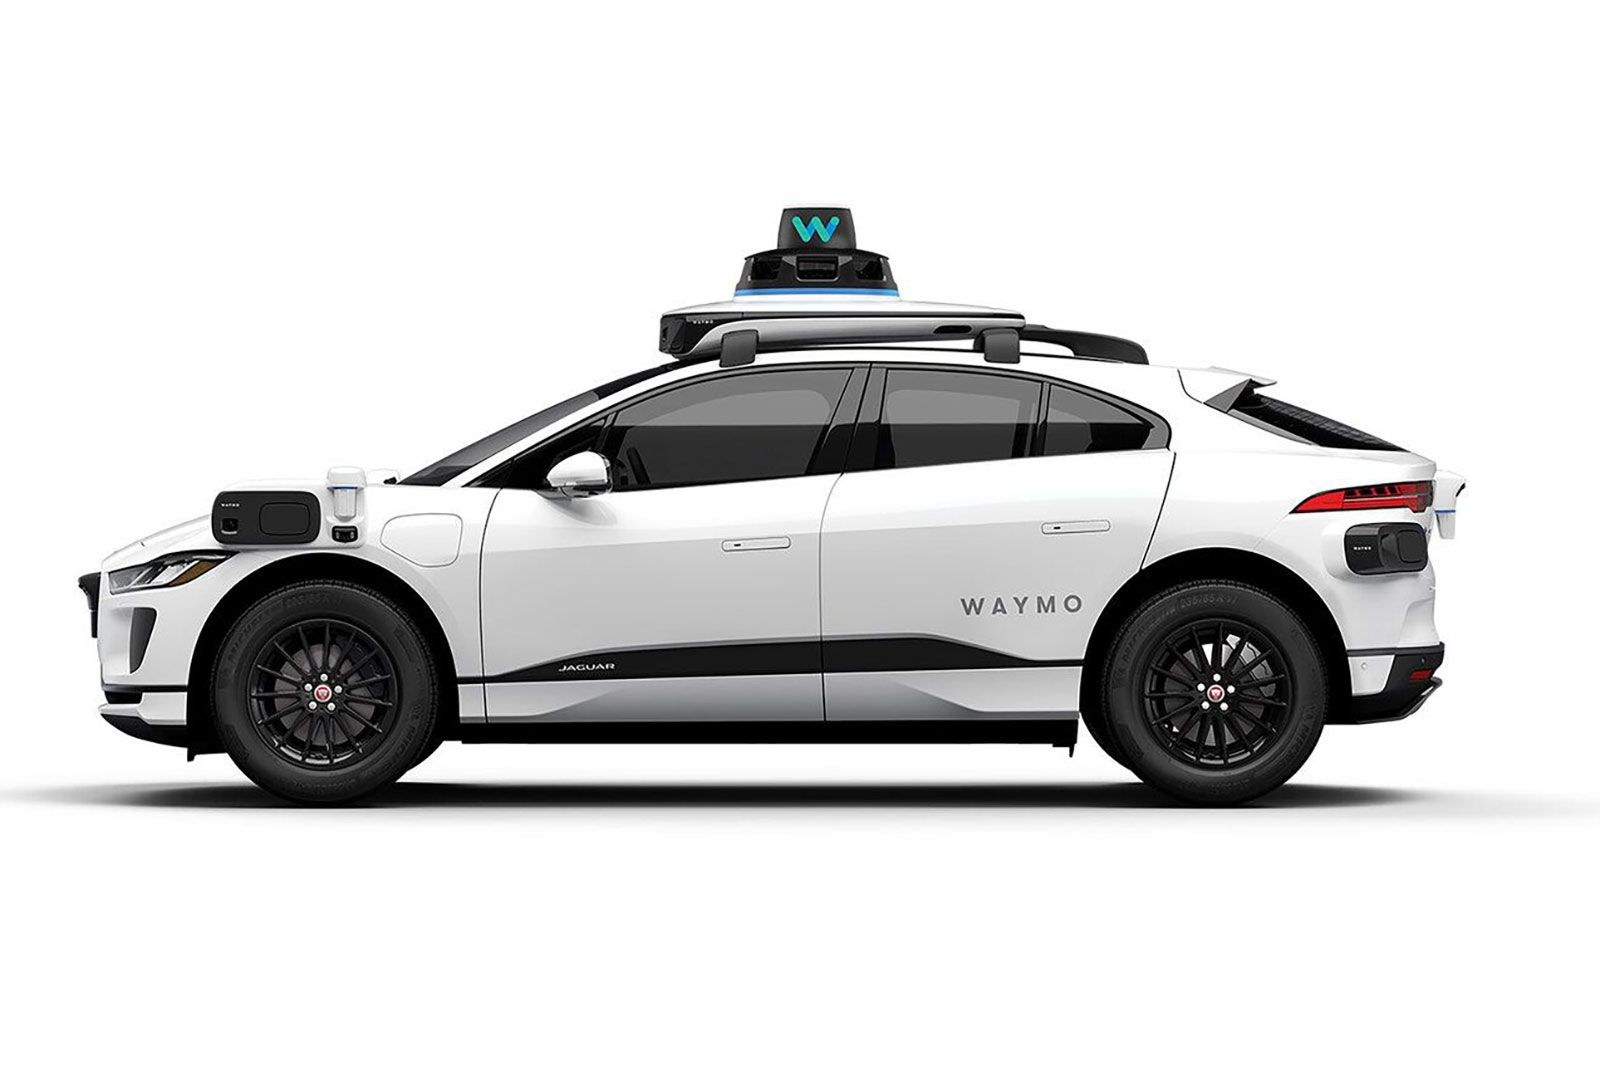
\includegraphics[height=2.6cm]{images/C13_3.jpg}
        \caption{Waymo}
    \end{subfigure}
    \hfill
    \begin{subfigure}[b]{0.24\textwidth}
        \centering
        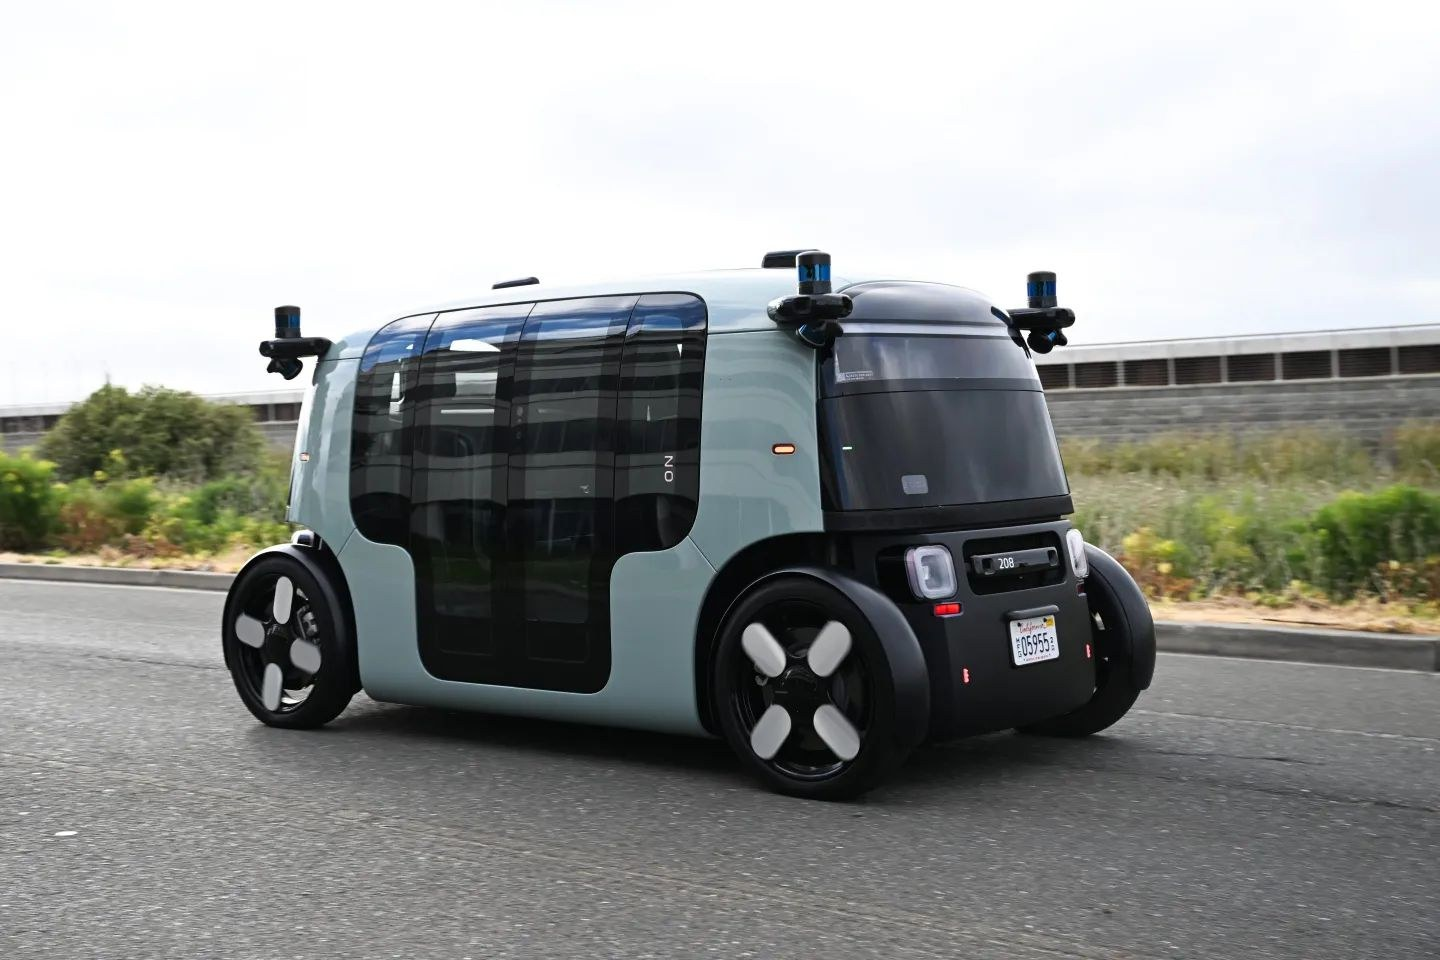
\includegraphics[height=2.6cm]{images/C13_4.jpg}
        \caption{Zoox}
    \end{subfigure}
    \hfill
    \begin{subfigure}[b]{0.28\textwidth}
        \centering
        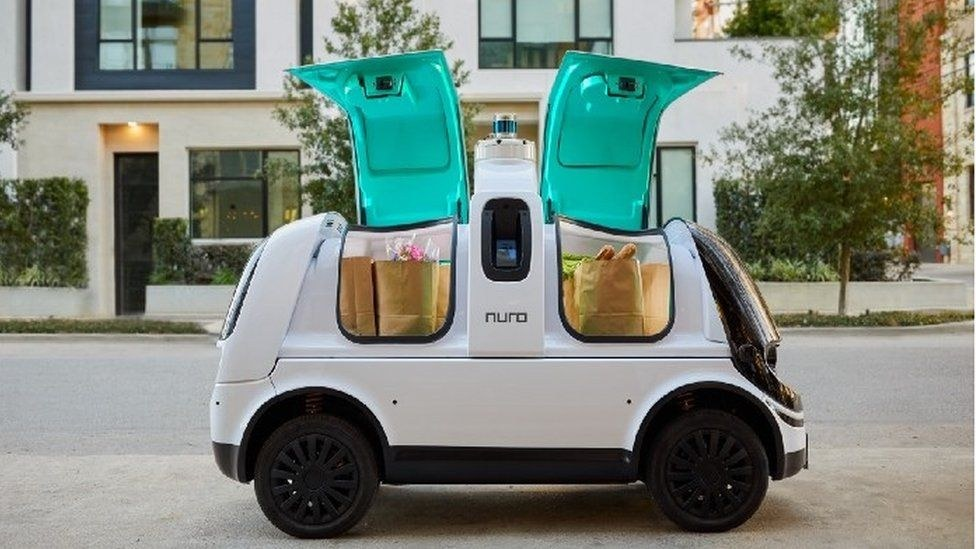
\includegraphics[height=2.6cm]{images/C13_5.jpg}
        \caption{Delivery vehicle}
    \end{subfigure}
    \hfill
    \begin{subfigure}[b]{0.18\textwidth}
        \centering
        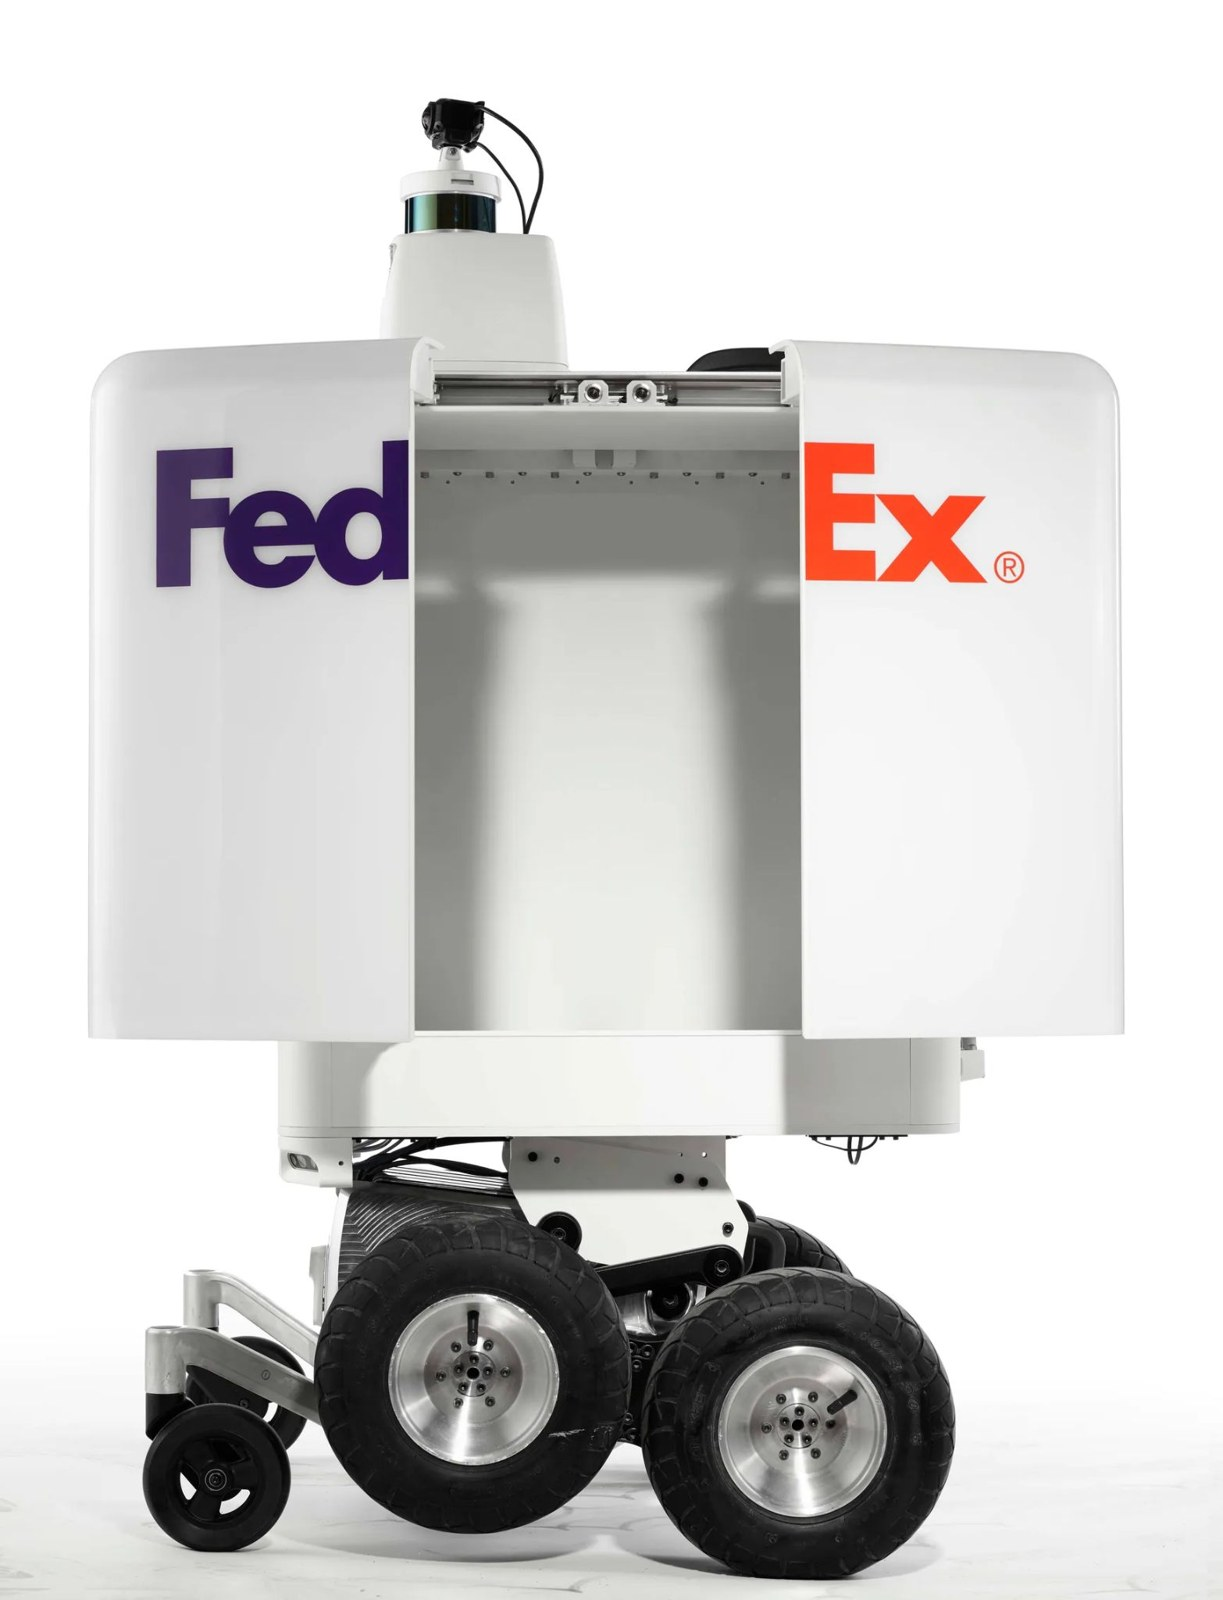
\includegraphics[height=2.6cm]{images/C13_6.jpg}
        \caption{Delivery robot}
    \end{subfigure}
    \caption{Robotaxis and last-minute delivery}
\end{figure}

\textbf{AGVs.} \textbf{Automated Guided Vehicles} are autonomous robots used in industry and logistics to transport materials in controlled environments such as warehouses and factories. They usually follow a \textbf{predefined path} and temporarily stop to avoid collisions.

\textbf{UGVs.} \textbf{Unmanned Ground Vehicles} are autonomous or remotely operated vehicles that perform tasks on the ground without humans on board. They are used in logistics, agriculture, search and rescue, and military applications.

\begin{figure}[H]
    \centering
    \begin{subfigure}[b]{0.45\textwidth}
        \centering
        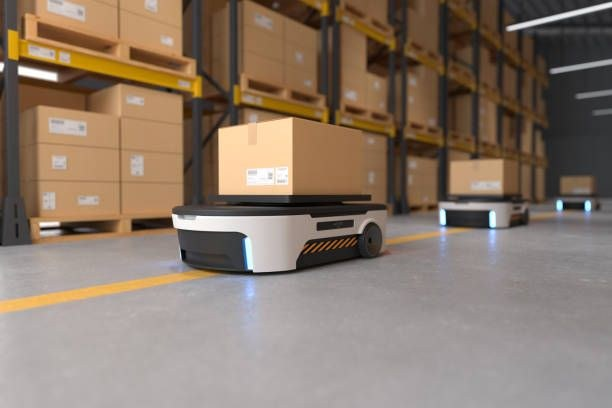
\includegraphics[height=3.3cm]{images/C13_7.jpg}
        \caption{AGV in a warehouse}
    \end{subfigure}
    \hfill
    \begin{subfigure}[b]{0.45\textwidth}
        \centering
        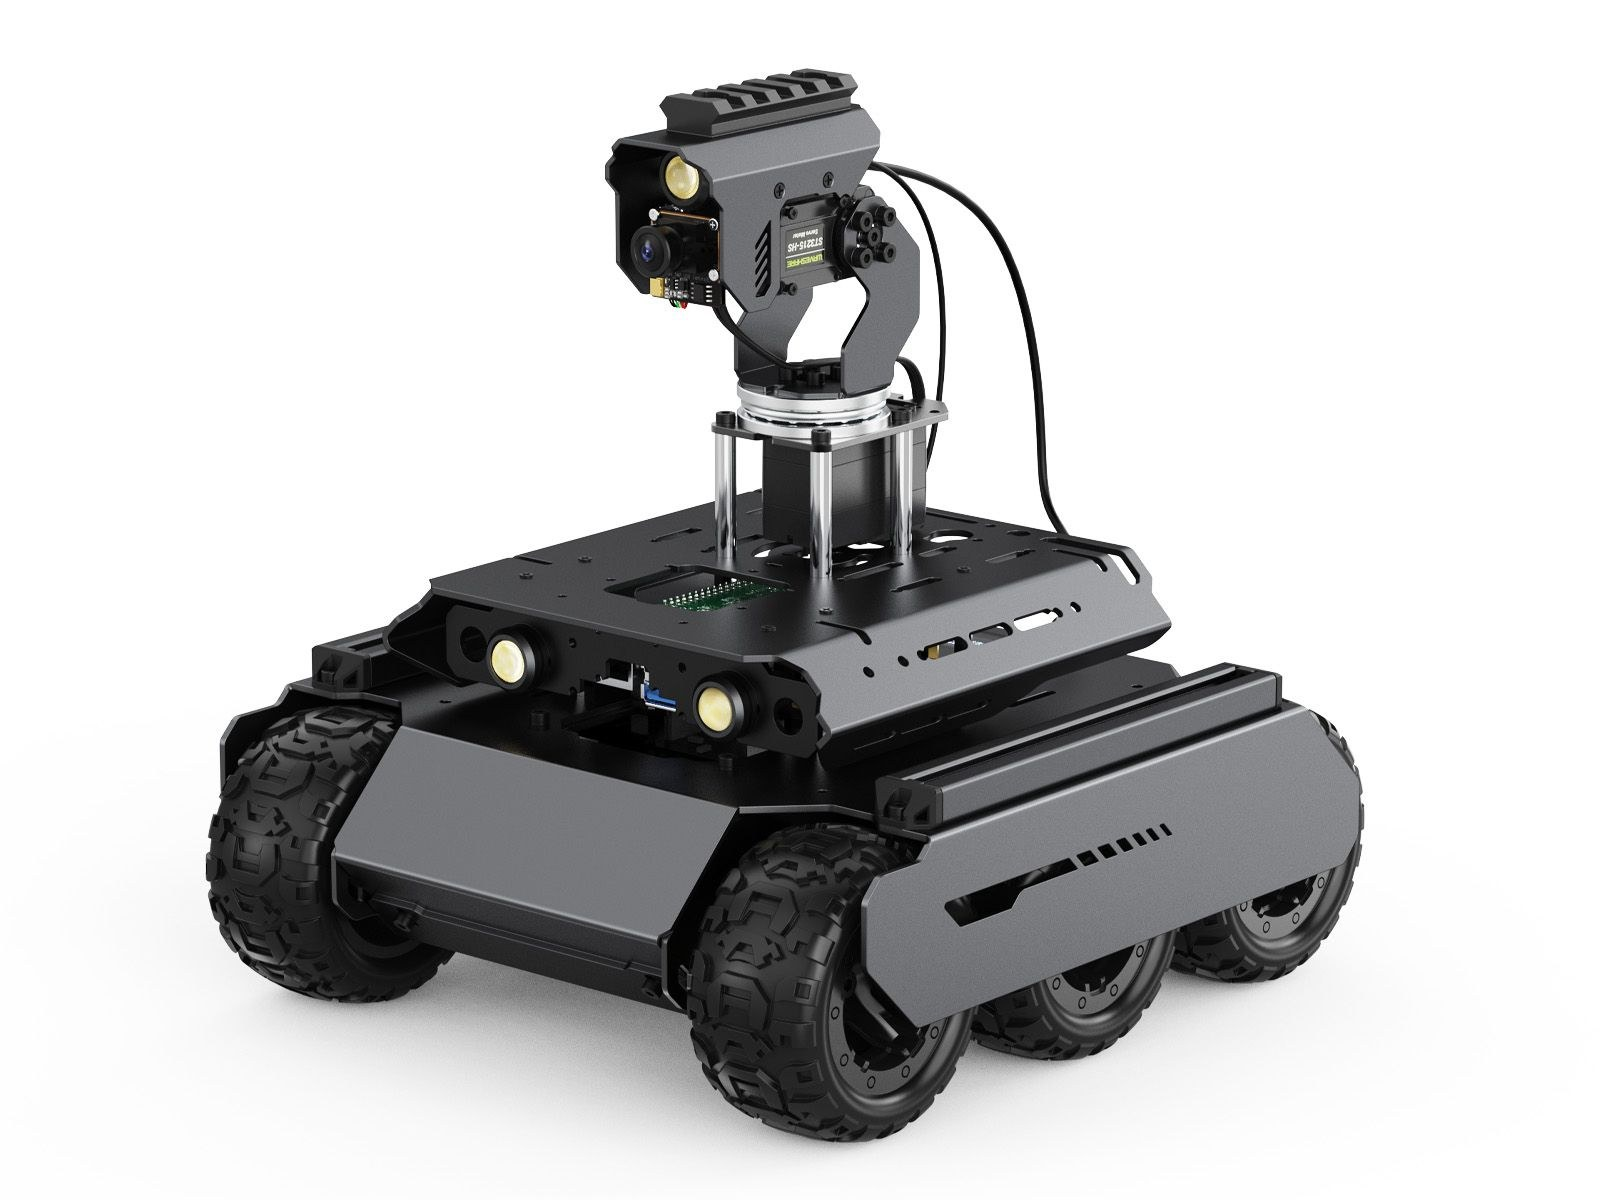
\includegraphics[height=3.3cm]{images/C13_8.jpg}
        \caption{UGV}
    \end{subfigure}
    \caption{AGVs and UGVs}
\end{figure}

\subsection{Unimore research projects on autonomous driving}
Unimore is involved in several autonomous driving projects:
\begin{compactitemize}
    \item \textbf{Autonomous Maserati and MASA} (Modena Automotive Smart Area), an urban area of Modena used to test autonomous cars;
    \item projects with \textbf{Poste Italiane} (autonomous delivery) and \textbf{Eni};
    \item \textbf{Roboracer} (also known as F1tenth), autonomous racing with 1:10 scale cars;
    \item \textbf{Formula Student Driverless} with the MMR Driverless team;
    \item the \textbf{Sensored F3}, an F3 car equipped with sensors;
    \item \textbf{Autonomous drone racing}.
\end{compactitemize}

\textbf{Unimore Racing} is the autonomous racing team, with about 25 members (PhD students, research assistants, master and bachelor students). It participates in the two main competitions for \textbf{full-scale autonomous racing}:
\begin{compactitemize}
    \item the \textbf{Indy Autonomous Challenge} (IAC), based on the Dallara Indy Lights car, at speeds of almost 290 km/h, with multi-vehicle overtaking competitions;
    \item the \textbf{Abu Dhabi Autonomous Racing League} (A2RL), based on the Dallara Super Formula. This car is more advanced: it has 4 independent brakes, high-performance actuators, high-end vehicle dynamics sensors and high downforce.
\end{compactitemize}

\begin{figure}[H]
    \centering
    \begin{subfigure}[b]{0.32\textwidth}
        \centering
        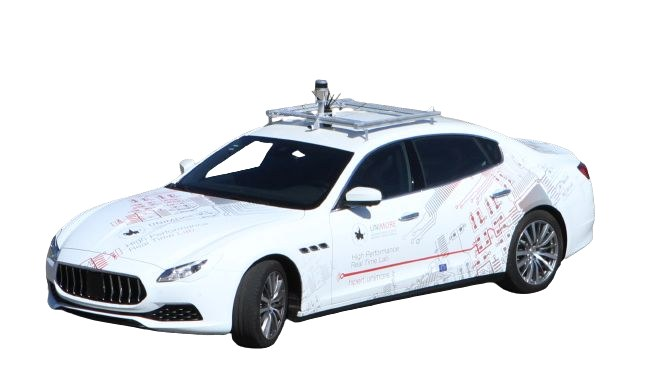
\includegraphics[height=2.7cm]{images/C13_9.jpg}
        \caption{Autonomous Maserati}
    \end{subfigure}
    \hfill
    \begin{subfigure}[b]{0.32\textwidth}
        \centering
        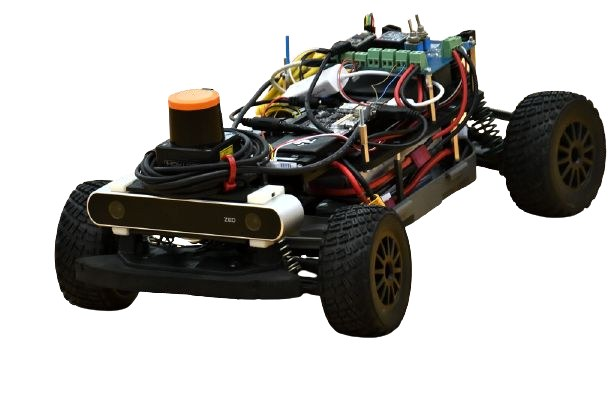
\includegraphics[height=2.7cm]{images/C13_10.jpg}
        \caption{Roboracer (F1tenth) car}
    \end{subfigure}
    \hfill
    \begin{subfigure}[b]{0.32\textwidth}
        \centering
        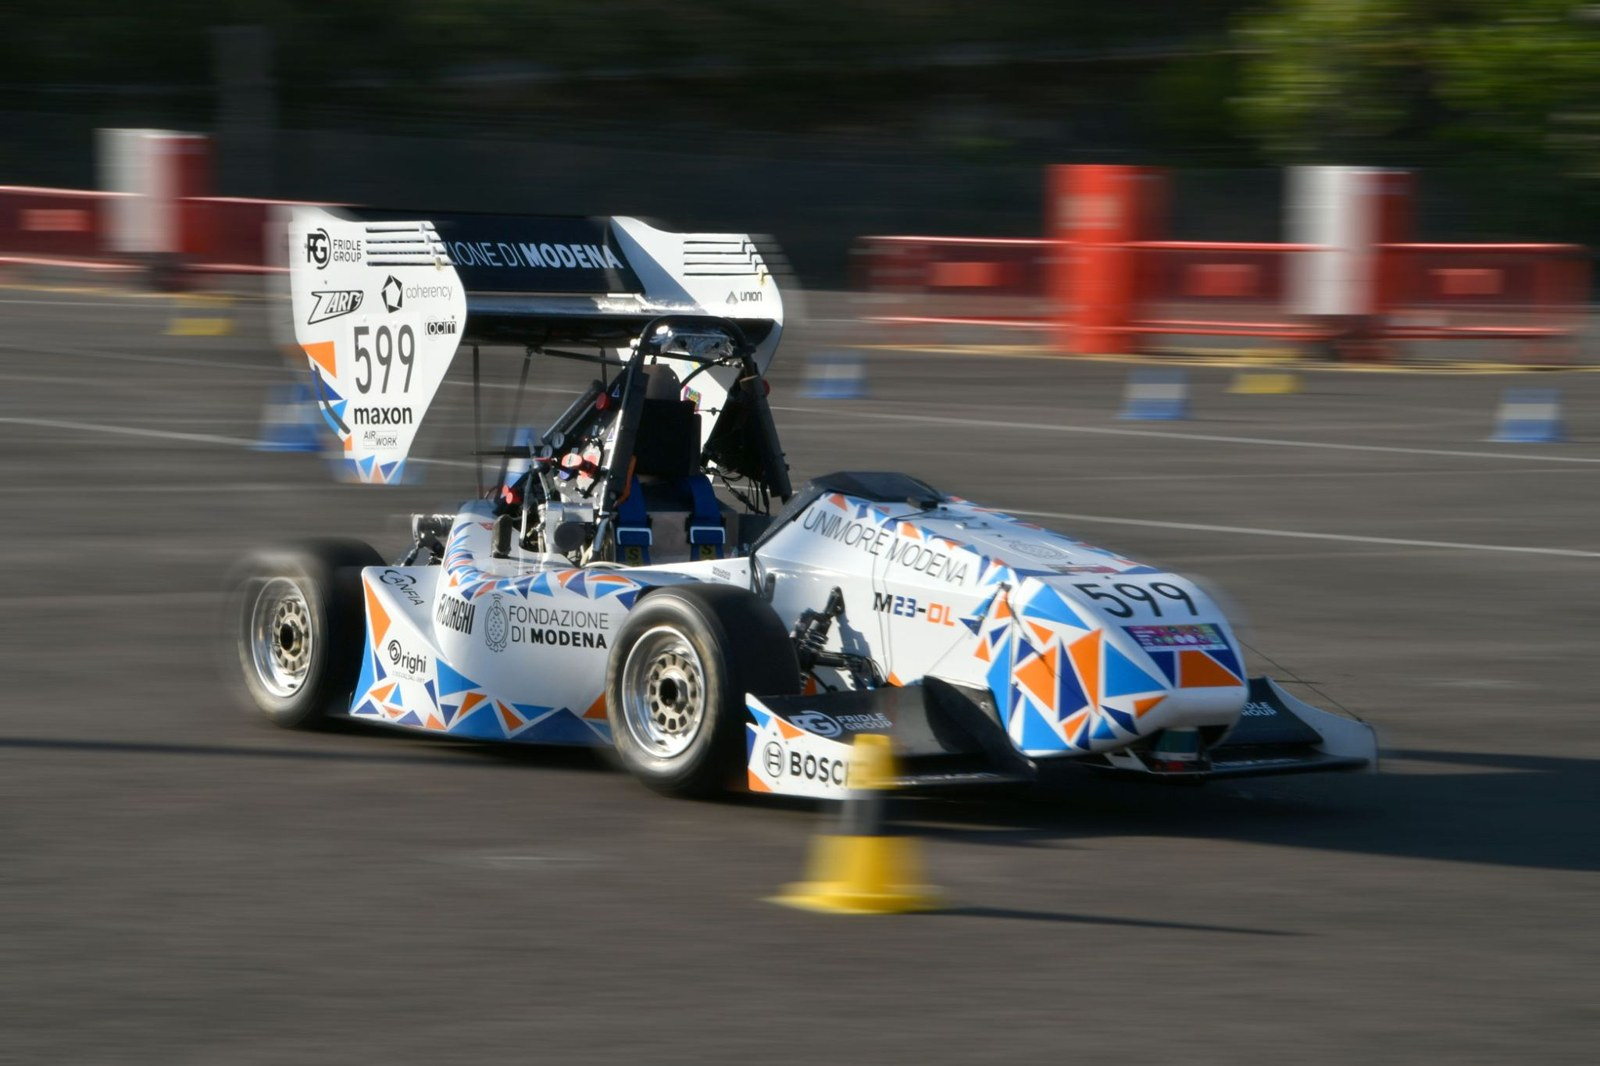
\includegraphics[height=2.7cm]{images/C13_11.jpg}
        \caption{Formula Student Driverless}
    \end{subfigure}

    \vspace{0.3cm}
    \begin{subfigure}[b]{0.45\textwidth}
        \centering
        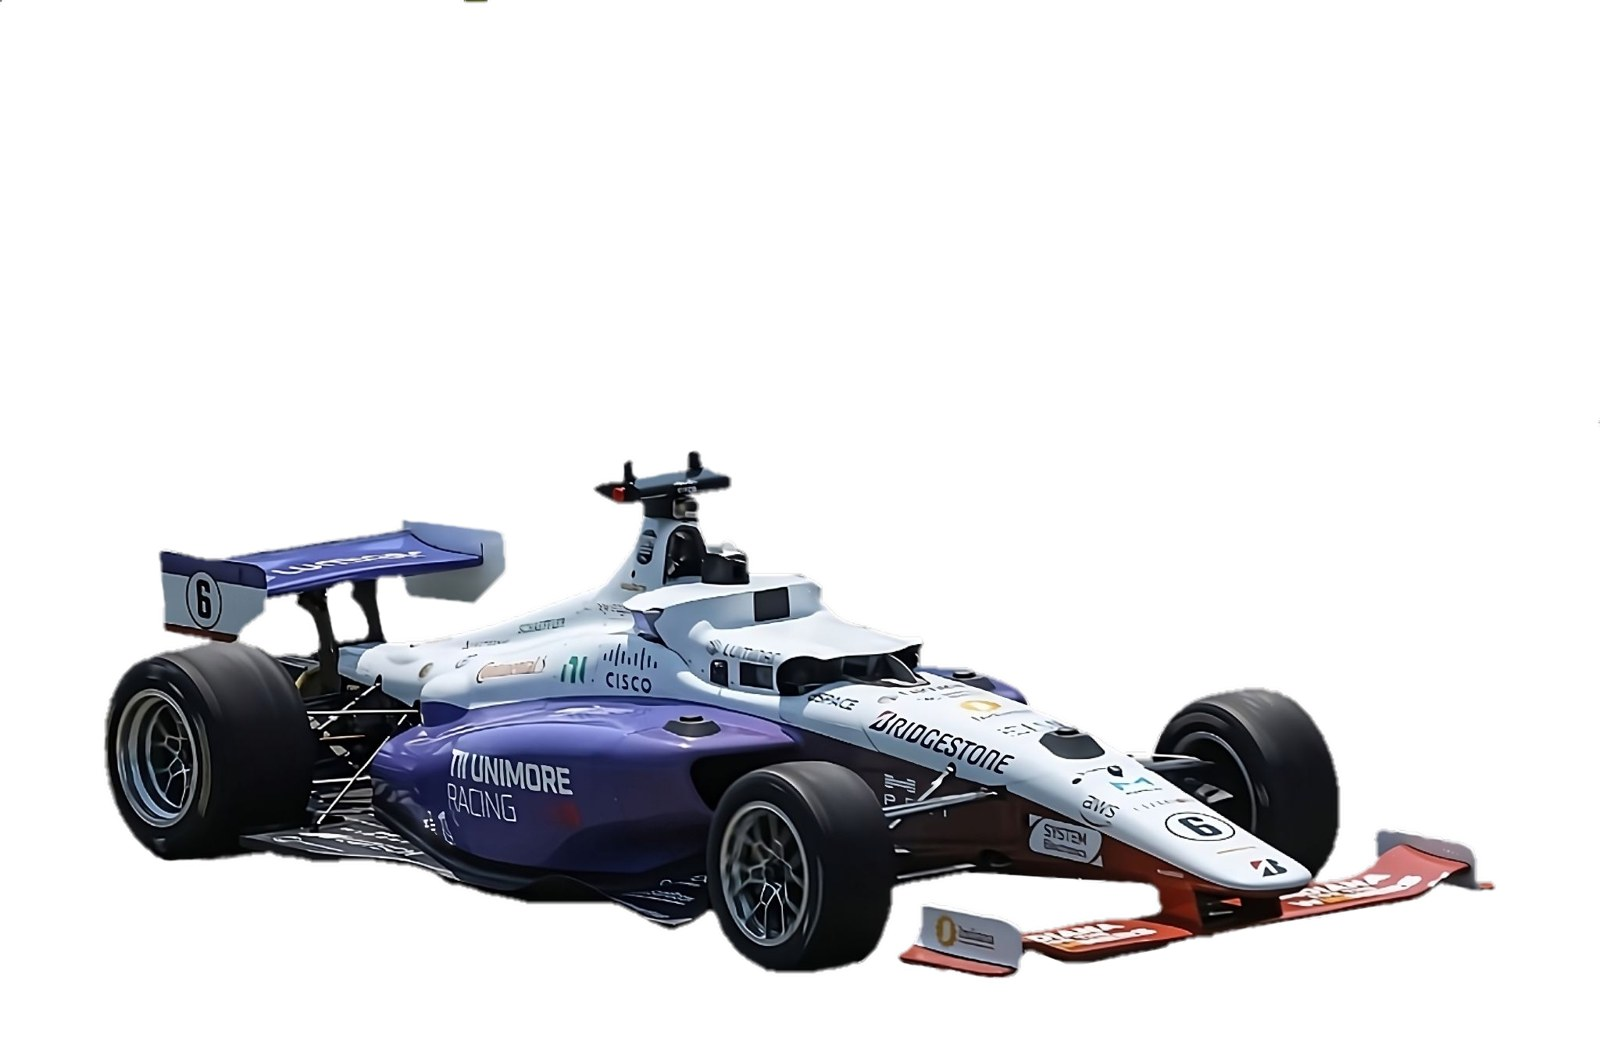
\includegraphics[height=3.2cm]{images/C13_12.jpg}
        \caption{IAC car (Dallara Indy Lights)}
    \end{subfigure}
    \hfill
    \begin{subfigure}[b]{0.45\textwidth}
        \centering
        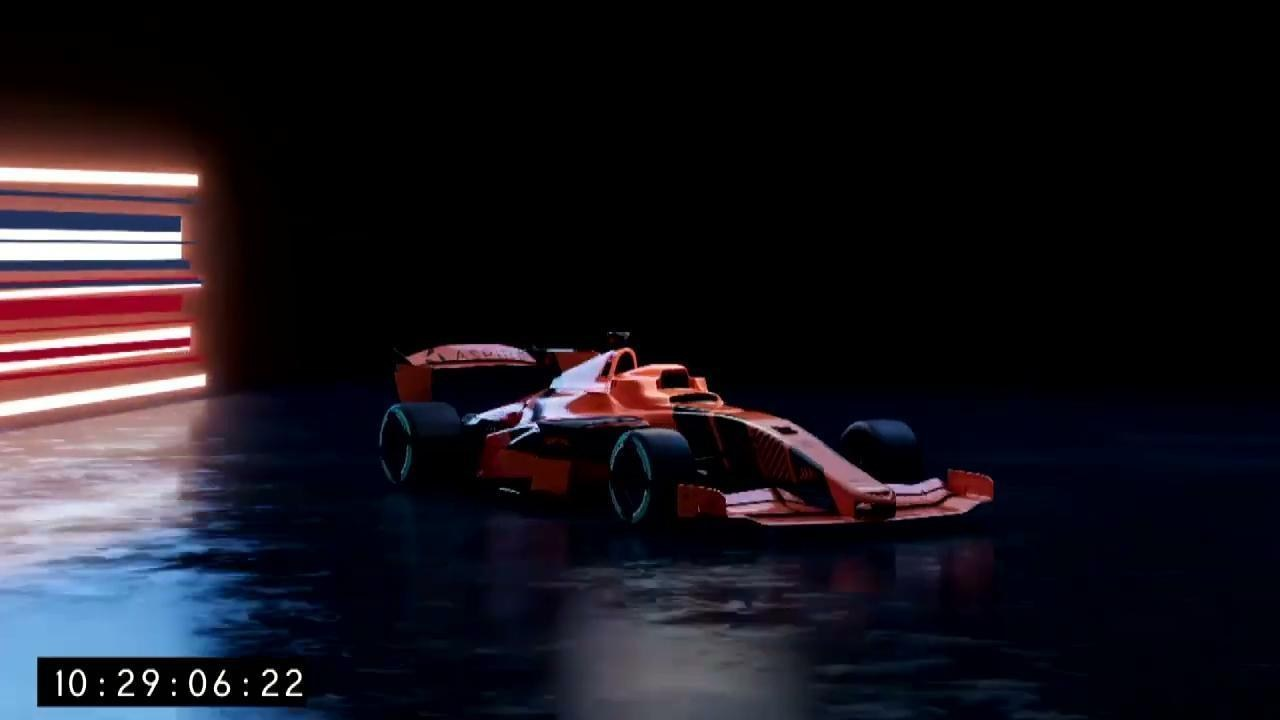
\includegraphics[height=3.2cm]{images/C13_13.jpg}
        \caption{A2RL car (Dallara Super Formula)}
    \end{subfigure}
    \caption{Some Unimore autonomous driving projects}
\end{figure}
